\PassOptionsToPackage{unicode=true}{hyperref} % options for packages loaded elsewhere
\PassOptionsToPackage{hyphens}{url}
%
\documentclass[]{book}
\usepackage{lmodern}
\usepackage{amssymb,amsmath}
\usepackage{ifxetex,ifluatex}
\usepackage{fixltx2e} % provides \textsubscript
\ifnum 0\ifxetex 1\fi\ifluatex 1\fi=0 % if pdftex
  \usepackage[T1]{fontenc}
  \usepackage[utf8]{inputenc}
  \usepackage{textcomp} % provides euro and other symbols
\else % if luatex or xelatex
  \usepackage{unicode-math}
  \defaultfontfeatures{Ligatures=TeX,Scale=MatchLowercase}
\fi
% use upquote if available, for straight quotes in verbatim environments
\IfFileExists{upquote.sty}{\usepackage{upquote}}{}
% use microtype if available
\IfFileExists{microtype.sty}{%
\usepackage[]{microtype}
\UseMicrotypeSet[protrusion]{basicmath} % disable protrusion for tt fonts
}{}
\IfFileExists{parskip.sty}{%
\usepackage{parskip}
}{% else
\setlength{\parindent}{0pt}
\setlength{\parskip}{6pt plus 2pt minus 1pt}
}
\usepackage{hyperref}
\hypersetup{
            pdftitle={Learning R for Clinical Trial Data},
            pdfauthor={Maya Gans},
            pdfborder={0 0 0},
            breaklinks=true}
\urlstyle{same}  % don't use monospace font for urls
\usepackage{color}
\usepackage{fancyvrb}
\newcommand{\VerbBar}{|}
\newcommand{\VERB}{\Verb[commandchars=\\\{\}]}
\DefineVerbatimEnvironment{Highlighting}{Verbatim}{commandchars=\\\{\}}
% Add ',fontsize=\small' for more characters per line
\usepackage{framed}
\definecolor{shadecolor}{RGB}{248,248,248}
\newenvironment{Shaded}{\begin{snugshade}}{\end{snugshade}}
\newcommand{\AlertTok}[1]{\textcolor[rgb]{0.94,0.16,0.16}{#1}}
\newcommand{\AnnotationTok}[1]{\textcolor[rgb]{0.56,0.35,0.01}{\textbf{\textit{#1}}}}
\newcommand{\AttributeTok}[1]{\textcolor[rgb]{0.77,0.63,0.00}{#1}}
\newcommand{\BaseNTok}[1]{\textcolor[rgb]{0.00,0.00,0.81}{#1}}
\newcommand{\BuiltInTok}[1]{#1}
\newcommand{\CharTok}[1]{\textcolor[rgb]{0.31,0.60,0.02}{#1}}
\newcommand{\CommentTok}[1]{\textcolor[rgb]{0.56,0.35,0.01}{\textit{#1}}}
\newcommand{\CommentVarTok}[1]{\textcolor[rgb]{0.56,0.35,0.01}{\textbf{\textit{#1}}}}
\newcommand{\ConstantTok}[1]{\textcolor[rgb]{0.00,0.00,0.00}{#1}}
\newcommand{\ControlFlowTok}[1]{\textcolor[rgb]{0.13,0.29,0.53}{\textbf{#1}}}
\newcommand{\DataTypeTok}[1]{\textcolor[rgb]{0.13,0.29,0.53}{#1}}
\newcommand{\DecValTok}[1]{\textcolor[rgb]{0.00,0.00,0.81}{#1}}
\newcommand{\DocumentationTok}[1]{\textcolor[rgb]{0.56,0.35,0.01}{\textbf{\textit{#1}}}}
\newcommand{\ErrorTok}[1]{\textcolor[rgb]{0.64,0.00,0.00}{\textbf{#1}}}
\newcommand{\ExtensionTok}[1]{#1}
\newcommand{\FloatTok}[1]{\textcolor[rgb]{0.00,0.00,0.81}{#1}}
\newcommand{\FunctionTok}[1]{\textcolor[rgb]{0.00,0.00,0.00}{#1}}
\newcommand{\ImportTok}[1]{#1}
\newcommand{\InformationTok}[1]{\textcolor[rgb]{0.56,0.35,0.01}{\textbf{\textit{#1}}}}
\newcommand{\KeywordTok}[1]{\textcolor[rgb]{0.13,0.29,0.53}{\textbf{#1}}}
\newcommand{\NormalTok}[1]{#1}
\newcommand{\OperatorTok}[1]{\textcolor[rgb]{0.81,0.36,0.00}{\textbf{#1}}}
\newcommand{\OtherTok}[1]{\textcolor[rgb]{0.56,0.35,0.01}{#1}}
\newcommand{\PreprocessorTok}[1]{\textcolor[rgb]{0.56,0.35,0.01}{\textit{#1}}}
\newcommand{\RegionMarkerTok}[1]{#1}
\newcommand{\SpecialCharTok}[1]{\textcolor[rgb]{0.00,0.00,0.00}{#1}}
\newcommand{\SpecialStringTok}[1]{\textcolor[rgb]{0.31,0.60,0.02}{#1}}
\newcommand{\StringTok}[1]{\textcolor[rgb]{0.31,0.60,0.02}{#1}}
\newcommand{\VariableTok}[1]{\textcolor[rgb]{0.00,0.00,0.00}{#1}}
\newcommand{\VerbatimStringTok}[1]{\textcolor[rgb]{0.31,0.60,0.02}{#1}}
\newcommand{\WarningTok}[1]{\textcolor[rgb]{0.56,0.35,0.01}{\textbf{\textit{#1}}}}
\usepackage{longtable,booktabs}
% Fix footnotes in tables (requires footnote package)
\IfFileExists{footnote.sty}{\usepackage{footnote}\makesavenoteenv{longtable}}{}
\usepackage{graphicx,grffile}
\makeatletter
\def\maxwidth{\ifdim\Gin@nat@width>\linewidth\linewidth\else\Gin@nat@width\fi}
\def\maxheight{\ifdim\Gin@nat@height>\textheight\textheight\else\Gin@nat@height\fi}
\makeatother
% Scale images if necessary, so that they will not overflow the page
% margins by default, and it is still possible to overwrite the defaults
% using explicit options in \includegraphics[width, height, ...]{}
\setkeys{Gin}{width=\maxwidth,height=\maxheight,keepaspectratio}
\setlength{\emergencystretch}{3em}  % prevent overfull lines
\providecommand{\tightlist}{%
  \setlength{\itemsep}{0pt}\setlength{\parskip}{0pt}}
\setcounter{secnumdepth}{5}
% Redefines (sub)paragraphs to behave more like sections
\ifx\paragraph\undefined\else
\let\oldparagraph\paragraph
\renewcommand{\paragraph}[1]{\oldparagraph{#1}\mbox{}}
\fi
\ifx\subparagraph\undefined\else
\let\oldsubparagraph\subparagraph
\renewcommand{\subparagraph}[1]{\oldsubparagraph{#1}\mbox{}}
\fi

% set default figure placement to htbp
\makeatletter
\def\fps@figure{htbp}
\makeatother

\usepackage{booktabs}
\usepackage{amsthm}
\makeatletter
\def\thm@space@setup{%
  \thm@preskip=8pt plus 2pt minus 4pt
  \thm@postskip=\thm@preskip
}
\makeatother
\usepackage[]{natbib}
\bibliographystyle{apalike}

\title{Learning R for Clinical Trial Data}
\author{Maya Gans}
\date{2020-03-12}

\begin{document}
\maketitle

{
\setcounter{tocdepth}{1}
\tableofcontents
}
\hypertarget{preface}{%
\chapter{Preface}\label{preface}}

This book is geared towards people who are bravely taking the step towards learning R but have yet to even download R on their local machines.

\hypertarget{the-book-will-walk-you-through}{%
\section{The book will walk you through:}\label{the-book-will-walk-you-through}}

\begin{itemize}
\tightlist
\item
  Getting R Set up on your computer
\item
  Understanding the RStudio IDE
\item
  Using the RStudio IDE
\item
  A gentle introduction to R
\item
  Importing and viewing data
\item
  Manipulating data
\item
  Visualizing data
\item
  Use the generated tables and plots to create a report
\end{itemize}

\hypertarget{getting-set-up-with-r}{%
\chapter{Getting Set Up with R}\label{getting-set-up-with-r}}

\hypertarget{setup-instructions}{%
\section{Setup instructions}\label{setup-instructions}}

R and RStudio are separate downloads and installations. R is the underlying statistical computing environment, but using R alone is no fun. RStudio is a graphical integrated development environment (IDE) that makes using R much easier and more interactive. You need to install R before you install RStudio. After installing both programs, you will need to install the \texttt{tidyverse} and \texttt{haven} packages from within RStudio. Follow the instructions below for your operating system, and then follow the instructions to install \texttt{tidyverse} and \texttt{haven}.

\hypertarget{windows}{%
\subsection{Windows}\label{windows}}

If you already have R and RStudio installed
Open RStudio, and click on ``Help'' \textgreater{} ``Check for updates''. If a new version is available, quit RStudio, and download the latest version for RStudio.
To check which version of R you are using, start RStudio and the first thing that appears in the console indicates the version of R you are running. Alternatively, you can type sessionInfo(), which will also display which version of R you are running. Go on the CRAN website and check whether a more recent version is available. If so, please download and install it. You can check here for more information on how to remove old versions from your system if you wish to do so.

If you don't have R and RStudio installed:

\begin{itemize}
\tightlist
\item
  Download R from the CRAN website.
\item
  Run the .exe file that was just downloaded
\item
  Go to the RStudio download page
\item
  Under Installers select RStudio x.yy.zzz - Windows Vista/7/8/10 (where x, y, and z represent version numbers)
\item
  Double click the file to install it
\end{itemize}

Once it's installed, open RStudio to make sure it works and you don't get any error messages.

\hypertarget{macos}{%
\subsection{macOS}\label{macos}}

If you already have R and RStudio installed
Open RStudio, and click on ``Help'' \textgreater{} ``Check for updates''. If a new version is available, quit RStudio, and download the latest version for RStudio.

To check the version of R you are using, start RStudio and the first thing that appears on the terminal indicates the version of R you are running. Alternatively, you can type sessionInfo(), which will also display which version of R you are running. Go on the CRAN website and check whether a more recent version is available. If so, please download and install it.

If you don't have R and RStudio installed:

\begin{itemize}
\tightlist
\item
  Download R from the CRAN website.
\item
  Select the .pkg file for the latest R version
\item
  Double click on the downloaded file to install R
\item
  It is also a good idea to install XQuartz (needed by some packages)
\item
  Go to the RStudio download page
\item
  Under Installers select RStudio x.yy.zzz - Mac OS X 10.6+ (64-bit) (where x, y, and z represent version numbers)
\item
  Double click the file to install RStudio
\end{itemize}

Once it's installed, open RStudio to make sure it works and you don't get any error messages.

\hypertarget{linux}{%
\section{Linux}\label{linux}}

Follow the instructions for your distribution from CRAN, they provide information to get the most recent version of R for common distributions. For most distributions, you could use your package manager (e.g., for Debian/Ubuntu run sudo apt-get install r-base, and for Fedora sudo yum install R), but we don't recommend this approach as the versions provided by this are usually out of date. In any case, make sure you have at least R 3.3.1.

\begin{itemize}
\tightlist
\item
  Go to the RStudio download page
\item
  Under Installers select the version that matches your distribution, and install it with your preferred method (e.g., with Debian/Ubuntu sudo dpkg -i rstudio-x.yy.zzz-amd64.deb at the terminal).
\item
  Once it's installed, open RStudio to make sure it works and you don't get any error messages.
\end{itemize}

\hypertarget{for-everyone}{%
\section{For everyone}\label{for-everyone}}

After installing R and RStudio, you need to install the \texttt{tidyverse} and \texttt{haven} packages.

After starting RStudio, at the console type:

\begin{verbatim}
install.packages(c("tidyverse", "haven"))
\end{verbatim}

You can also do this by going to Tools -\textgreater{} Install Packages and typing the names of the packages separated by a comma.

\hypertarget{intro}{%
\chapter{RStudio IDE}\label{intro}}

The RStudio IDE open-source product is free under the Affero General Public License (AGPL) v3. The RStudio IDE is also available with a commercial license and priority email support from RStudio, Inc.

We will use RStudio IDE to write code, navigate the files on our computer, inspect the variables we are going to create, and visualize the plots we will generate. RStudio can also be used for other things (e.g., version control, developing packages, writing Shiny apps) that will not be covered in this book.

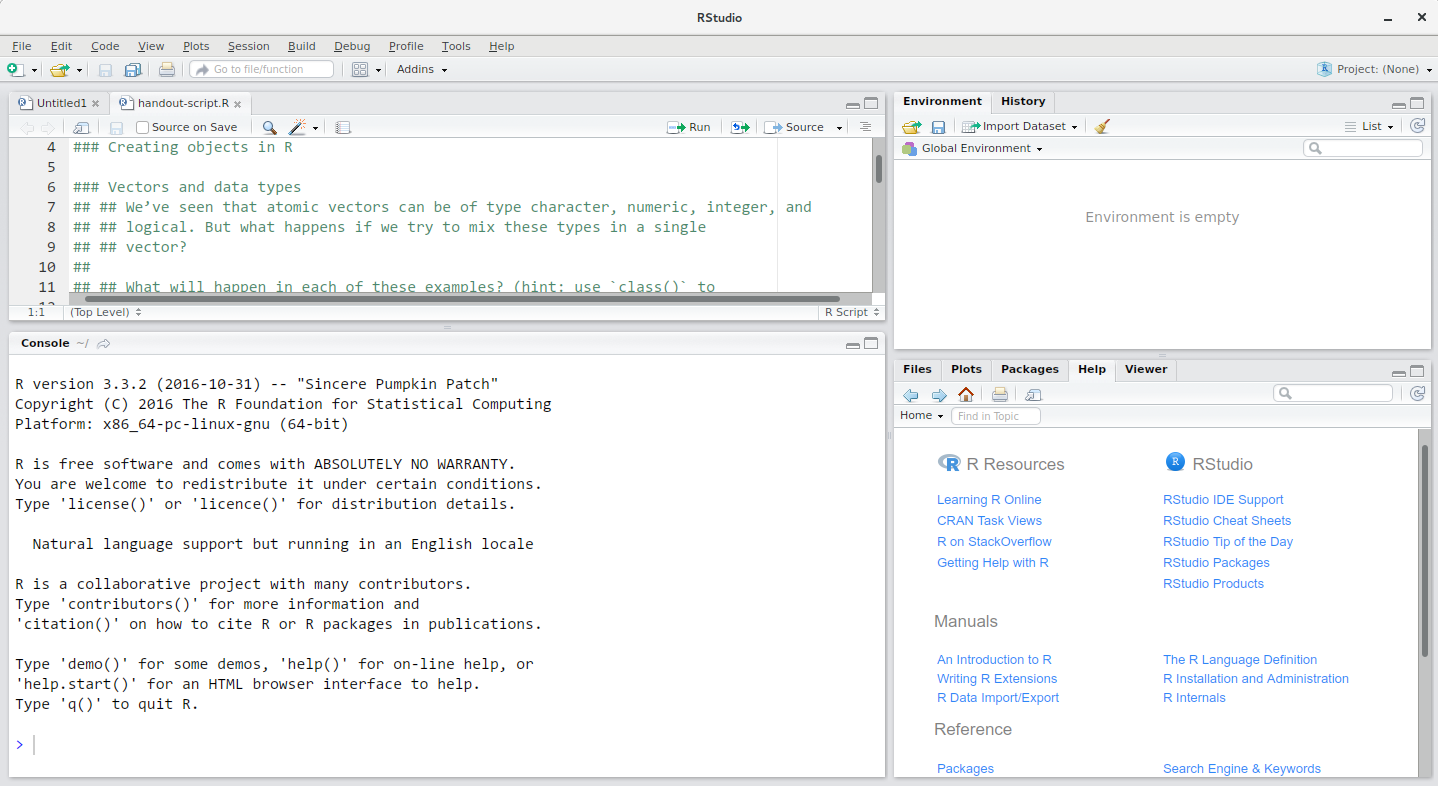
\includegraphics[width=19.97in]{/Users/mayagans/Desktop/Cytel_Bookdown/bookdown-demo-master/_book/bookdown-demo_files/figure-html/rstudio-screenshot}

RStudio is divided into 4 ``Panes'':

\begin{enumerate}
\def\labelenumi{\arabic{enumi})}
\tightlist
\item
  The Source for your scripts and documents (top-left, in the default layout),
\item
  Your Environment/History (top-right)
\item
  Your Files/Plots/Packages/Help/Viewer (bottom-right)
\item
  The R Console (bottom-left).
\end{enumerate}

The placement of these panes and their content can be customized (see menu, Tools -\textgreater{} Global Options -\textgreater{} Pane Layout).

One of the advantages of using RStudio is that all the information you need to write code is available in a single window. Additionally, with many shortcuts, autocompletion, and highlighting for the major file types you use while developing in R, RStudio will make typing easier and less error-prone.

\hypertarget{getting-set-up}{%
\section{Getting set up}\label{getting-set-up}}

It is good practice to keep a set of related data, analyses, and text self-contained in a single folder, called the working directory. All of the scripts within this folder can then use relative paths to files that indicate where inside the project a file is located (as opposed to absolute paths, which point to where a file is on a specific computer). Working this way makes it a lot easier to move your project around on your computer and share it with others without worrying about whether or not the underlying scripts will still work.

RStudio provides a helpful set of tools to do this through its ``Projects'' interface, which not only creates a working directory for you, but also remembers its location (allowing you to quickly navigate to it) and optionally preserves custom settings and open files to make it easier to resume work after a break. Go through the steps for creating an ``R Project'' for this tutorial below.

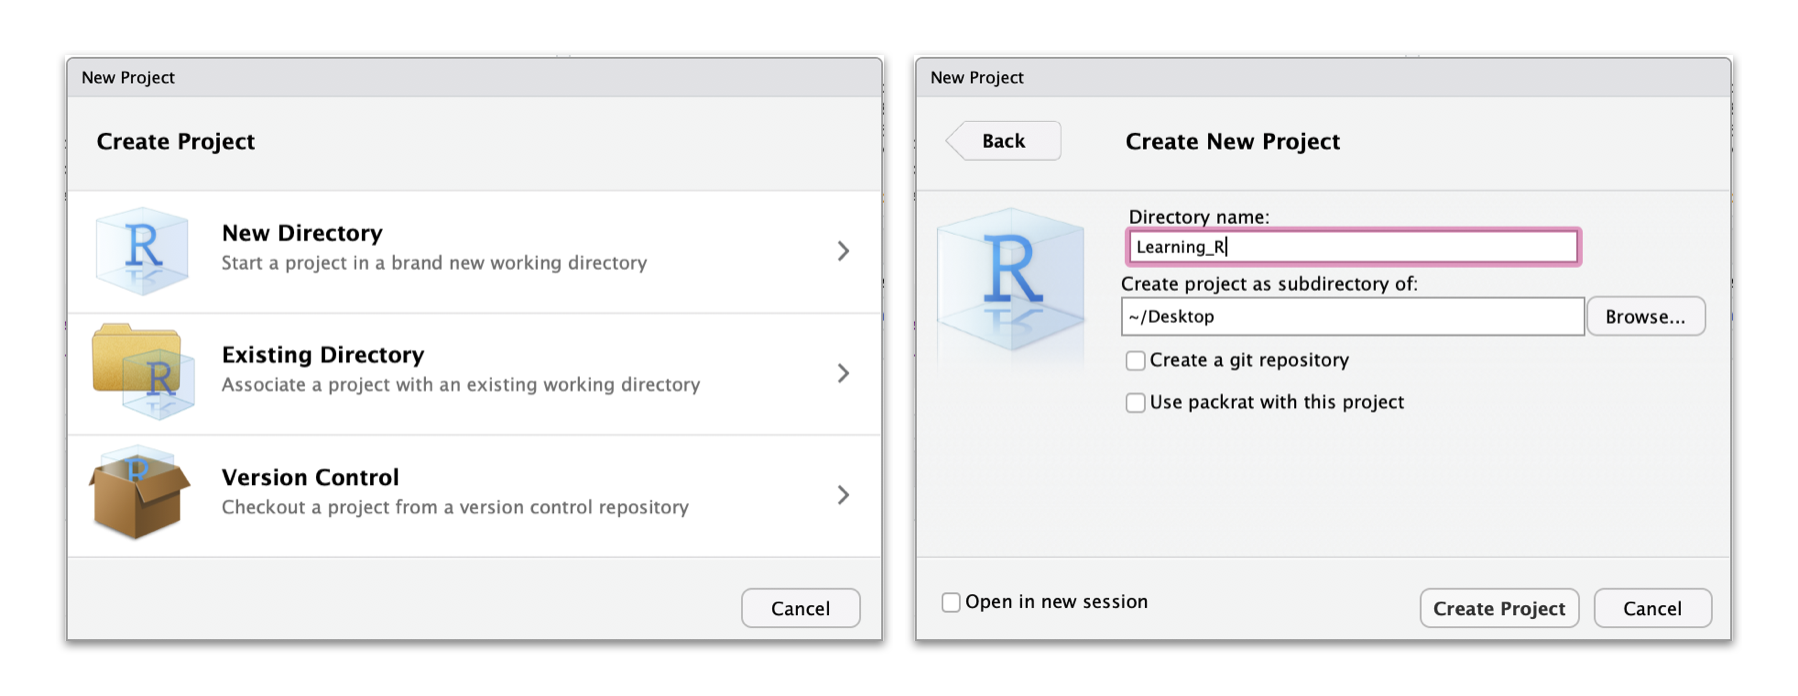
\includegraphics[width=24.97in]{/Users/mayagans/Desktop/Cytel_Bookdown/bookdown-demo-master/_book/bookdown-demo_files/figure-html/rstudio-newproject}

\hypertarget{start-rstudio.}{%
\section{Start RStudio.}\label{start-rstudio.}}

\begin{itemize}
\tightlist
\item
  Under the File menu, click on New Project.
\item
  Choose New Directory, then New Project.
\item
  Enter a name for this new folder (or ``directory''), and choose a convenient location for it.
\item
  Click on Create Project.
\end{itemize}

\hypertarget{optional-preferences}{%
\section{Optional Preferences}\label{optional-preferences}}

RStudio's default preferences generally work well, but saving a workspace to .RData can be cumbersome, especially if you are working with larger datasets. To turn that off, go to Tools --\textgreater{} `Global Options' and select the `Never' option for `Save workspace to .RData' on exit.' This step is optional, but if you love something it's sometimes best to let it go.

\begin{center}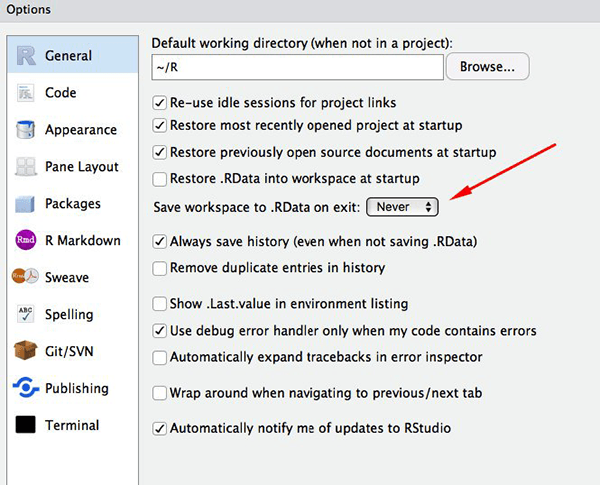
\includegraphics[width=8.33in]{/Users/mayagans/Desktop/Cytel_Bookdown/bookdown-demo-master/_book/bookdown-demo_files/figure-html/rstudio-preferences} \end{center}

\hypertarget{organizing-your-working-directory}{%
\section{Organizing your working directory}\label{organizing-your-working-directory}}

Using a consistent folder structure across your projects will help keep things organized, and will also make it easy to find/file things in the future. This can be especially helpful when you have multiple projects. In general, you may create directories (folders) for scripts, data, and documents.

\begin{itemize}
\tightlist
\item
  data\_raw/
\item
  data/
\end{itemize}

Use these folders to store raw data and intermediate datasets you may create for the need of a particular analysis. For the sake of transparency and provenance, you should always keep a copy of your raw data accessible and do as much of your data cleanup and preprocessing programmatically (i.e., with scripts, rather than manually) as possible.

\begin{itemize}
\tightlist
\item
  report.Rmd
\end{itemize}

We will be using an RMarkdown file to create our report. This allows for inline coding with plot and table outputs. We are going to keep the report in the root of our working directory because we are only going to use one file and it will make things easier. Outside of this demonstraition you'd most likely create a folder of reports and title them accordingly.

\begin{itemize}
\tightlist
\item
  Additional (sub)directories depending on your project needs (like scripts and functions)
\end{itemize}

We will need a \texttt{data\_raw/} folder for our demo project to store our raw \texttt{sas7bdat} files, and we will use \texttt{data/} for when we learn how to export data as CSV files, and a \texttt{report.Rmd} file for our generated report containing figures and tables.

Under the Files tab on the right of the screen, click on New Folder and create a folder named data\_raw within your newly created working directory (e.g., \textasciitilde{}/cdisc-demo/). (Alternatively, type dir.create(``data\_raw'') at your R console.)

Repeat these operations to create a data folder. Under the Files tab you can click New File then RMarkdown and create the \texttt{report.Rmd}.

Your working directory should now look like this:

\begin{center}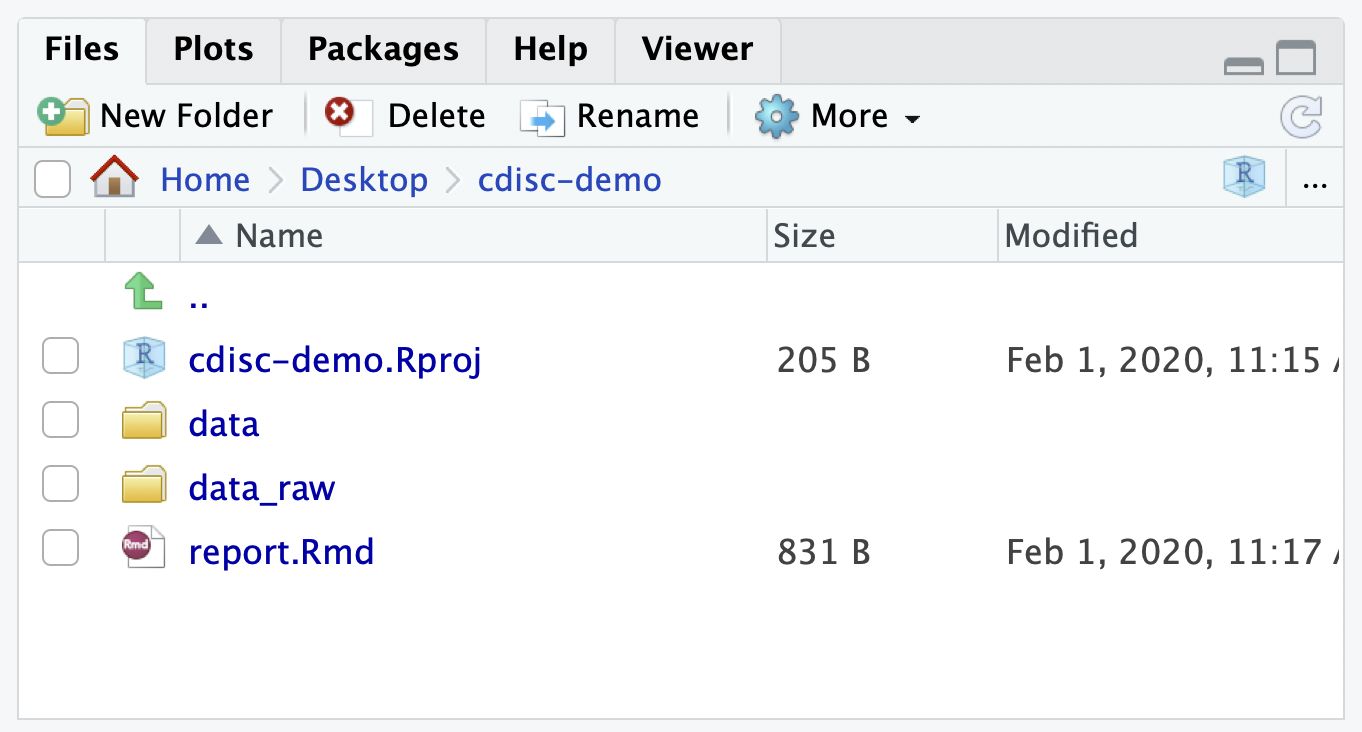
\includegraphics[width=18.92in]{/Users/mayagans/Desktop/Cytel_Bookdown/bookdown-demo-master/_book/bookdown-demo_files/figure-html/rstudio-filestructure} \end{center}

\hypertarget{exercise}{%
\section{Exercise}\label{exercise}}

Download the ADSL and ADAE from XYZ and add it to your \texttt{raw\_data} folder

\hypertarget{interacting-with-r}{%
\chapter{Interacting with R}\label{interacting-with-r}}

The basis of programming is that we write down instructions for the computer to follow, and then we tell the computer to follow those instructions. We write, or code, instructions in R because it is a common language that both the computer and we can understand. We call the instructions commands and we tell the computer to follow the instructions by executing (also called running) those commands.

There are two main ways of interacting with R: by using the console or by using script files (plain text files that contain your code). The console pane (in RStudio, the bottom left panel) is the place where commands written in the R language can be typed and executed immediately by the computer. It is also where the results will be shown for commands that have been executed. You can type commands directly into the console and press Enter to execute those commands, but they will be forgotten when you close the session.

Because we want our code and workflow to be reproducible, it is better to type the commands we want in the script editor, and save the script. This way, there is a complete record of what we did, and anyone (including our future selves!) can easily replicate the results on their computer.

RStudio allows you to execute commands directly from the script editor by using the \texttt{Ctrl\ +\ Enter} shortcut (on Macs, \texttt{Cmd\ +\ Return} will work, too). The command on the current line in the script (indicated by the cursor) or all of the commands in the currently selected text will be sent to the console and executed when you press Ctrl + Enter. You can find other keyboard shortcuts in this RStudio cheatsheet about the RStudio IDE.

At some point in your analysis you may want to check the content of a variable or the structure of an object, without necessarily keeping a record of it in your script. You can type these commands and execute them directly in the console. RStudio provides the Ctrl + 1 and Ctrl + 2 shortcuts allow you to jump between the script and the console panes.

If R is ready to accept commands, the R console shows a \textgreater{} prompt. If it receives a command (by typing, copy-pasting or sent from the script editor using Ctrl + Enter), R will try to execute it, and when ready, will show the results and come back with a new \textgreater{} prompt to wait for new commands.

If R is still waiting for you to enter more data because it isn't complete yet, the console will show a + prompt. It means that you haven't finished entering a complete command. This is because you have not `closed' a parenthesis or quotation, i.e.~you don't have the same number of left-parentheses as right-parentheses, or the same number of opening and closing quotation marks. When this happens, and you thought you finished typing your command, click inside the console window and press Esc; this will cancel the incomplete command and return you to the \textgreater{} prompt.

\hypertarget{seeking-help}{%
\section{Seeking help}\label{seeking-help}}

Use the built-in RStudio help interface to search for more information on R functions
RStudio help interface. This panel by default can be found at the lower right hand panel of RStudio. As seen in the screenshot, by typing the word ``Mean'', RStudio tries to also give a number of suggestions that you might be interested in. The description is then shown in the display window.

If you need help with a specific function, let's say \texttt{barplot()}, you can type: \texttt{?barplot}

If you just need to remind yourself of the names of the arguments, you can use:
\texttt{args(lm)}

If you are looking for a function to do a particular task, you can use the help.search() function, which is called by the double question mark \texttt{??}. However, this only looks through the installed packages for help pages with a match to your search request

If you can't find what you are looking for, you can use the rdocumentation.org website that searches through the help files across all packages available.

Finally, a generic Google or internet search \texttt{R\ \textless{}task\textgreater{}} will often either send you to the appropriate package documentation or a helpful forum where someone else has already asked your question.

\hypertarget{introduction-to-r}{%
\chapter{Introduction to R}\label{introduction-to-r}}

\hypertarget{learning-objectives}{%
\section{Learning Objectives}\label{learning-objectives}}

\begin{itemize}
\tightlist
\item
  Define the following terms as they relate to R: object, assign, call, function, arguments, options.
\item
  Assign values to objects in R.
\item
  Learn how to name objects
\item
  Use comments to inform script.
\item
  Solve simple arithmetic operations in R.
\item
  Call functions and use arguments to change their default options.
\item
  Inspect the content of vectors and manipulate their content.
\item
  Subset and extract values from vectors.
\item
  Analyze vectors with missing data.
\end{itemize}

\hypertarget{creating-objects-in-r}{%
\section{Creating objects in R}\label{creating-objects-in-r}}

You can get output from R simply by typing math in the console:

\begin{Shaded}
\begin{Highlighting}[]
\DecValTok{3} \OperatorTok{+}\StringTok{ }\DecValTok{5}
\end{Highlighting}
\end{Shaded}

\begin{verbatim}
## [1] 8
\end{verbatim}

However, to do useful and interesting things, we need to assign values to objects. To create an object, we need to give it a name followed by the assignment operator \textless{}-, and the value we want to give it:

\begin{Shaded}
\begin{Highlighting}[]
\NormalTok{weight_kg <-}\StringTok{ }\DecValTok{55}
\end{Highlighting}
\end{Shaded}

\texttt{\textless{}-} is the assignment operator. It assigns values on the right to objects on the left. So, after executing \texttt{x\ \textless{}-\ 3}, the value of \texttt{x} is \texttt{3}. The arrow can be read as 3 \textbf{goes into} \texttt{x}. For historical reasons, you can also use = for assignments, but not in every context. Because of the slight differences in syntax, it is good practice to always use \texttt{\textless{}-} for assignments.

In RStudio, typing \texttt{Alt\ +\ -} (push \texttt{Alt} at the same time as the \texttt{-} key) will write \texttt{\textless{}-} in a single keystroke in a PC, while typing \texttt{Option\ +\ -} (push \texttt{Option} at the same time as the \texttt{-} key) does the same in a Mac.

Objects can be given any name such as \texttt{x}, \texttt{current\_temperature}, or \texttt{subject\_id}. You want your object names to be explicit and not too long. They \textbf{cannot} start with a number (\texttt{2x} is not valid, but \texttt{x2} is). R is \textbf{case sensitive} (e.g., \texttt{weight\_kg} is different from \texttt{Weight\_kg}).

There are some names that cannot be used because they are the names of fundamental functions in R (e.g., \texttt{if}, \texttt{else}, \texttt{for}). In general, even if it's allowed, it's best to not use other function names (e.g., \texttt{c}, \texttt{T}, \texttt{mean}, \texttt{data}, \texttt{df}, \texttt{weights}).

If in doubt, check the help to see if the name is already in use. It's also best to avoid dots (.) within an object name as in my.dataset. There are many functions in R with dots in their names for historical reasons, but because dots have a special meaning in R (for methods) and other programming languages, it's best to avoid them.

It is also recommended to use nouns for object names, and verbs for function names. It's important to be consistent in the styling of your code (where you put spaces, how you name objects, etc.). Using a consistent coding style makes your code clearer to read for your future self and your collaborators. In R, three popular style guides are \href{https://google.github.io/styleguide/Rguide.html}{Google's}, \href{\%5Bhttp://jef.works/R-style-guide/}{Jean Fan's} and the \href{https://style.tidyverse.org/}{tidyverse's}. You can install the \texttt{lintr} package to automatically check for issues in the styling of your code.

\hypertarget{objects-vs.variables}{%
\subsection{Objects vs.~variables}\label{objects-vs.variables}}

What are known as objects in R are known as variables in many other programming languages. Depending on the context, object and variable can have drastically different meanings. However, in this lesson, the two words are used synonymously.

When assigning a value to an object, R does not print anything. You can force R to print the value by using parentheses or by typing the object name:

\begin{Shaded}
\begin{Highlighting}[]
\NormalTok{weight_kg <-}\StringTok{ }\DecValTok{55}  \CommentTok{# doesn't print anything}
\end{Highlighting}
\end{Shaded}

\begin{Shaded}
\begin{Highlighting}[]
\NormalTok{(weight_kg <-}\StringTok{ }\DecValTok{55}\NormalTok{)  }\CommentTok{# but putting parenthesis around the call prints the value of `weight_kg`}
\end{Highlighting}
\end{Shaded}

\begin{verbatim}
## [1] 55
\end{verbatim}

\begin{Shaded}
\begin{Highlighting}[]
\NormalTok{weight_kg }\CommentTok{# and so does typing the name of the object}
\end{Highlighting}
\end{Shaded}

\begin{verbatim}
## [1] 55
\end{verbatim}

Now that R has \texttt{weight\_kg} in memory, we can do arithmetic with it. For instance, we may want to convert this weight into pounds (weight in pounds is 2.2 times the weight in kg):

\begin{Shaded}
\begin{Highlighting}[]
\FloatTok{2.2} \OperatorTok{*}\StringTok{ }\NormalTok{weight_kg}
\end{Highlighting}
\end{Shaded}

\begin{verbatim}
## [1] 121
\end{verbatim}

We can also change an object's value by assigning it a new one:

\begin{Shaded}
\begin{Highlighting}[]
\NormalTok{weight_kg <-}\StringTok{ }\FloatTok{57.5}
\FloatTok{2.2} \OperatorTok{*}\StringTok{ }\NormalTok{weight_kg}
\end{Highlighting}
\end{Shaded}

\begin{verbatim}
## [1] 126.5
\end{verbatim}

This means that assigning a value to one object does not change the values of other objects For example, let's store the animal's weight in pounds in a new object, weight\_lb:

\begin{Shaded}
\begin{Highlighting}[]
\NormalTok{weight_lb <-}\StringTok{ }\FloatTok{2.2} \OperatorTok{*}\StringTok{ }\NormalTok{weight_kg}
\end{Highlighting}
\end{Shaded}

and then change \texttt{weight\_kg} to 100.

\begin{Shaded}
\begin{Highlighting}[]
\NormalTok{weight_kg <-}\StringTok{ }\DecValTok{100}
\end{Highlighting}
\end{Shaded}

\hypertarget{comments}{%
\subsection{Comments}\label{comments}}

The comment character in R is \#, anything to the right of a \# in a script will be ignored by R. It is useful to leave notes and explanations in your scripts. RStudio makes it easy to comment or uncomment a paragraph: after selecting the lines you want to comment, press at the same time on your keyboard \texttt{Ctrl\ +\ Shift\ +\ C}. If you only want to comment out one line, you can put the cursor at any location of that line (i.e.~no need to select the whole line), then press \texttt{Ctrl\ +\ Shift\ +\ C}.

\hypertarget{functions-and-their-arguments}{%
\subsection{Functions and their arguments}\label{functions-and-their-arguments}}

Functions are ``canned scripts'' that automate more complicated sets of commands including operations assignments, etc. Many functions are predefined, or can be made available by importing R packages (more on that later). A function usually takes one or more inputs called arguments. Functions often (but not always) return a value. A typical example would be the function sqrt(). The input (the argument) must be a number, and the return value (in fact, the output) is the square root of that number. Executing a function (`running it') is called calling the function. An example of a function call is:

\begin{verbatim}
b <- sqrt(a)
\end{verbatim}

Here, the value of \texttt{a} is given to the \texttt{sqrt()} function, the \texttt{sqrt()} function calculates the square root, and returns the value which is then assigned to the object \texttt{b}. This function is very simple, because it takes just one argument.

The return `value' of a function need not be numerical (like that of \texttt{sqrt()}), and it also does not need to be a single item: it can be a set of things, or even a dataset. We'll see that when we read data files into R.

Arguments can be anything, not only numbers or filenames, but also other objects. Exactly what each argument means differs per function, and must be looked up in the documentation. Some functions take arguments which may either be specified by the user, or, if left out, take on a default value: these are called options. Options are typically used to alter the way the function operates, such as whether it ignores `bad values', or what symbol to use in a plot. However, if you want something specific, you can specify a value of your choice which will be used instead of the default.

Let's try a function that can take multiple arguments: \texttt{round()}.

\begin{Shaded}
\begin{Highlighting}[]
\KeywordTok{round}\NormalTok{(}\FloatTok{3.14159}\NormalTok{)}
\end{Highlighting}
\end{Shaded}

\begin{verbatim}
## [1] 3
\end{verbatim}

Here, we've called \texttt{round()} with just one argument, \texttt{3.14159}, and it has returned the value \texttt{3}. That's because the default is to round to the nearest whole number. If we want more digits we can see how to do that by getting information about the round function. We can use \texttt{args(round)} to find what arguments it takes, or look at the help for this function using \texttt{?round}.

\begin{Shaded}
\begin{Highlighting}[]
\KeywordTok{args}\NormalTok{(round)}
\end{Highlighting}
\end{Shaded}

\begin{verbatim}
## function (x, digits = 0) 
## NULL
\end{verbatim}

\begin{Shaded}
\begin{Highlighting}[]
\NormalTok{?round}
\end{Highlighting}
\end{Shaded}

We see that if we want a different number of digits, we can type \texttt{digits\ =\ 2} or however many we want.

\begin{Shaded}
\begin{Highlighting}[]
\KeywordTok{round}\NormalTok{(}\FloatTok{3.14159}\NormalTok{, }\DataTypeTok{digits =} \DecValTok{2}\NormalTok{)}
\end{Highlighting}
\end{Shaded}

\begin{verbatim}
## [1] 3.14
\end{verbatim}

If you provide the arguments in the exact same order as they are defined you don't have to name them:

\begin{Shaded}
\begin{Highlighting}[]
\KeywordTok{round}\NormalTok{(}\FloatTok{3.14159}\NormalTok{, }\DecValTok{2}\NormalTok{)}
\end{Highlighting}
\end{Shaded}

\begin{verbatim}
## [1] 3.14
\end{verbatim}

And if you do name the arguments, you can switch their order:

\begin{Shaded}
\begin{Highlighting}[]
\KeywordTok{round}\NormalTok{(}\DataTypeTok{digits =} \DecValTok{2}\NormalTok{, }\DataTypeTok{x =} \FloatTok{3.14159}\NormalTok{)}
\end{Highlighting}
\end{Shaded}

\begin{verbatim}
## [1] 3.14
\end{verbatim}

It's good practice to put the non-optional arguments (like the number you're rounding) first in your function call, and to then specify the names of all optional arguments. If you don't, someone reading your code might have to look up the definition of a function with unfamiliar arguments to understand what you're doing.

\hypertarget{vectors-and-data-types}{%
\section{Vectors and data types}\label{vectors-and-data-types}}

A vector is the most common and basic data type in R, and is pretty much the workhorse of R. A vector is composed by a series of values, which can be either numbers or characters. We can assign a series of values to a vector using the \texttt{c()} function. For example we can create a vector of animal weights and assign it to a new object \texttt{weight\_g}:

\begin{Shaded}
\begin{Highlighting}[]
\NormalTok{weight_g <-}\StringTok{ }\KeywordTok{c}\NormalTok{(}\DecValTok{50}\NormalTok{, }\DecValTok{60}\NormalTok{, }\DecValTok{65}\NormalTok{, }\DecValTok{82}\NormalTok{)}
\NormalTok{weight_g}
\end{Highlighting}
\end{Shaded}

\begin{verbatim}
## [1] 50 60 65 82
\end{verbatim}

A vector can also contain characters:

\begin{Shaded}
\begin{Highlighting}[]
\NormalTok{animals <-}\StringTok{ }\KeywordTok{c}\NormalTok{(}\StringTok{"mouse"}\NormalTok{, }\StringTok{"rat"}\NormalTok{, }\StringTok{"dog"}\NormalTok{)}
\NormalTok{animals}
\end{Highlighting}
\end{Shaded}

\begin{verbatim}
## [1] "mouse" "rat"   "dog"
\end{verbatim}

The quotes around ``mouse'', ``rat'', etc. are essential here. Without the quotes R will assume objects have been created called \texttt{mouse}, \texttt{rat} and \texttt{dog}. As these objects don't exist in R's memory, there will be an error message.

There are many functions that allow you to inspect the content of a vector. \texttt{length()} tells you how many elements are in a particular vector:

\begin{Shaded}
\begin{Highlighting}[]
\KeywordTok{length}\NormalTok{(weight_g)}
\end{Highlighting}
\end{Shaded}

\begin{verbatim}
## [1] 4
\end{verbatim}

\begin{Shaded}
\begin{Highlighting}[]
\KeywordTok{length}\NormalTok{(animals)}
\end{Highlighting}
\end{Shaded}

\begin{verbatim}
## [1] 3
\end{verbatim}

An important feature of a vector, is that all of the elements are the same type of data. The function \texttt{class()} indicates the class (the type of element) of an object:

\begin{Shaded}
\begin{Highlighting}[]
\KeywordTok{class}\NormalTok{(weight_g)}
\end{Highlighting}
\end{Shaded}

\begin{verbatim}
## [1] "numeric"
\end{verbatim}

\begin{Shaded}
\begin{Highlighting}[]
\KeywordTok{class}\NormalTok{(animals)}
\end{Highlighting}
\end{Shaded}

\begin{verbatim}
## [1] "character"
\end{verbatim}

The function \texttt{str()} provides an overview of the structure of an object and its elements. It is a useful function when working with large and complex objects:

\begin{Shaded}
\begin{Highlighting}[]
\KeywordTok{str}\NormalTok{(weight_g)}
\end{Highlighting}
\end{Shaded}

\begin{verbatim}
##  num [1:4] 50 60 65 82
\end{verbatim}

\begin{Shaded}
\begin{Highlighting}[]
\KeywordTok{str}\NormalTok{(animals)}
\end{Highlighting}
\end{Shaded}

\begin{verbatim}
##  chr [1:3] "mouse" "rat" "dog"
\end{verbatim}

You can use the \texttt{c()} function to add other elements to your vector:

\begin{Shaded}
\begin{Highlighting}[]
\NormalTok{weight_g <-}\StringTok{ }\KeywordTok{c}\NormalTok{(weight_g, }\DecValTok{90}\NormalTok{) }\CommentTok{# add to the end of the vector}
\NormalTok{weight_g}
\end{Highlighting}
\end{Shaded}

\begin{verbatim}
## [1] 50 60 65 82 90
\end{verbatim}

\begin{Shaded}
\begin{Highlighting}[]
\NormalTok{weight_g <-}\StringTok{ }\KeywordTok{c}\NormalTok{(}\DecValTok{30}\NormalTok{, weight_g) }\CommentTok{# add to the beginning of the vector}
\NormalTok{weight_g}
\end{Highlighting}
\end{Shaded}

\begin{verbatim}
## [1] 30 50 60 65 82 90
\end{verbatim}

In the first line, we take the original vector \texttt{weight\_g}, add the value 90 to the end of it, and save the result back into \texttt{weight\_g}. Then we add the value 30 to the beginning, again saving the result back into \texttt{weight\_g}.

We can do this over and over again to grow a vector, or assemble a dataset. As we program, this may be useful to add results that we are collecting or calculating.

An \textbf{atomic vector} is the simplest R \textbf{data type} and is a linear vector of a single type. Above, we saw 2 of the 6 main atomic vector types that R uses: \texttt{"character"} and \texttt{"numeric"} (or \texttt{"double"}). These are the basic building blocks that all R objects are built from. The other 4 atomic vector types are:

\begin{itemize}
\tightlist
\item
  \texttt{"logical"} for \texttt{TRUE} and \texttt{FALSE} (the boolean data type)
\item
  \texttt{"integer"} for integer numbers (e.g., \texttt{2L}, the \texttt{L} indicates to R that it's an integer)
\item
  \texttt{"complex"} to represent complex numbers with real and imaginary parts (e.g., \texttt{1\ +\ 4i}) and that's all we're going to say about them
\item
  \texttt{"raw"} for bitstreams that we won't discuss further
\end{itemize}

You can check the type of your vector using the \texttt{typeof()} function and inputting your vector as the argument.

Vectors are one of the many data structures that R uses. Other important ones are lists (\texttt{list}), matrices (\texttt{matrix}), data frames (\texttt{data.frame}), factors (\texttt{factor}) and arrays (\texttt{array}).

\hypertarget{subsetting-vectors}{%
\section{Subsetting vectors}\label{subsetting-vectors}}

If we want to extract one or several values from a vector, we must provide one or several indices in square brackets. For instance:

\begin{Shaded}
\begin{Highlighting}[]
\NormalTok{animals <-}\StringTok{ }\KeywordTok{c}\NormalTok{(}\StringTok{"mouse"}\NormalTok{, }\StringTok{"rat"}\NormalTok{, }\StringTok{"dog"}\NormalTok{, }\StringTok{"cat"}\NormalTok{)}
\end{Highlighting}
\end{Shaded}

\begin{Shaded}
\begin{Highlighting}[]
\NormalTok{animals[}\DecValTok{2}\NormalTok{]}
\end{Highlighting}
\end{Shaded}

\begin{verbatim}
## [1] "rat"
\end{verbatim}

\begin{Shaded}
\begin{Highlighting}[]
\NormalTok{animals[}\KeywordTok{c}\NormalTok{(}\DecValTok{3}\NormalTok{, }\DecValTok{2}\NormalTok{)]}
\end{Highlighting}
\end{Shaded}

\begin{verbatim}
## [1] "dog" "rat"
\end{verbatim}

We can also repeat the indices to create an object with more elements than the original one:

\begin{Shaded}
\begin{Highlighting}[]
\NormalTok{more_animals <-}\StringTok{ }\NormalTok{animals[}\KeywordTok{c}\NormalTok{(}\DecValTok{1}\NormalTok{, }\DecValTok{2}\NormalTok{, }\DecValTok{3}\NormalTok{, }\DecValTok{2}\NormalTok{, }\DecValTok{1}\NormalTok{, }\DecValTok{4}\NormalTok{)]}
\NormalTok{more_animals}
\end{Highlighting}
\end{Shaded}

\begin{verbatim}
## [1] "mouse" "rat"   "dog"   "rat"   "mouse" "cat"
\end{verbatim}

R indices start at 1. Programming languages like Fortran, MATLAB, Julia, and R start counting at 1, because that's what human beings typically do. Languages in the C family (including C++, Java, Perl, and Python) count from 0 because that's simpler for computers to do.

\hypertarget{conditional-subsetting}{%
\subsection{Conditional subsetting}\label{conditional-subsetting}}

Another common way of subsetting is by using a logical vector. \texttt{TRUE} will select the element with the same index, while \texttt{FALSE} will not:

\begin{Shaded}
\begin{Highlighting}[]
\NormalTok{weight_g <-}\StringTok{ }\KeywordTok{c}\NormalTok{(}\DecValTok{21}\NormalTok{, }\DecValTok{34}\NormalTok{, }\DecValTok{39}\NormalTok{, }\DecValTok{54}\NormalTok{, }\DecValTok{55}\NormalTok{)}
\NormalTok{weight_g[}\KeywordTok{c}\NormalTok{(}\OtherTok{TRUE}\NormalTok{, }\OtherTok{FALSE}\NormalTok{, }\OtherTok{TRUE}\NormalTok{, }\OtherTok{TRUE}\NormalTok{, }\OtherTok{FALSE}\NormalTok{)]}
\end{Highlighting}
\end{Shaded}

\begin{verbatim}
## [1] 21 39 54
\end{verbatim}

Typically, these logical vectors are not typed by hand, but are the output of other functions or logical tests. For instance, if you wanted to select only the values above 50:

\begin{Shaded}
\begin{Highlighting}[]
\NormalTok{weight_g }\OperatorTok{>}\StringTok{ }\DecValTok{50}   \CommentTok{# will return logicals with TRUE for the indices that meet the condition}
\end{Highlighting}
\end{Shaded}

\begin{verbatim}
## [1] FALSE FALSE FALSE  TRUE  TRUE
\end{verbatim}

So we can use this to select only the values above 50

\begin{Shaded}
\begin{Highlighting}[]
\NormalTok{weight_g[weight_g }\OperatorTok{>}\StringTok{ }\DecValTok{50}\NormalTok{]}
\end{Highlighting}
\end{Shaded}

\begin{verbatim}
## [1] 54 55
\end{verbatim}

You can combine multiple tests using \& (both conditions are true, AND) or \textbar{} (at least one of the conditions is true, OR):

\begin{Shaded}
\begin{Highlighting}[]
\NormalTok{weight_g[weight_g }\OperatorTok{<}\StringTok{ }\DecValTok{30} \OperatorTok{|}\StringTok{ }\NormalTok{weight_g }\OperatorTok{>}\StringTok{ }\DecValTok{50}\NormalTok{]}
\end{Highlighting}
\end{Shaded}

\begin{verbatim}
## [1] 21 54 55
\end{verbatim}

\begin{Shaded}
\begin{Highlighting}[]
\NormalTok{weight_g[weight_g }\OperatorTok{>=}\StringTok{ }\DecValTok{30} \OperatorTok{&}\StringTok{ }\NormalTok{weight_g }\OperatorTok{==}\StringTok{ }\DecValTok{21}\NormalTok{]}
\end{Highlighting}
\end{Shaded}

\begin{verbatim}
## numeric(0)
\end{verbatim}

Here, \texttt{\textless{}} stands for ``less than'', \texttt{\textgreater{}} for ``greater than'', \texttt{\textgreater{}=} for ``greater than or equal to'', and \texttt{==} for ``equal to''. The double equal sign \texttt{==} is a test for numerical equality between the left and right hand sides, and should not be confused with the single \texttt{=} sign, which performs variable assignment (similar to \texttt{\textless{}-}).

A common task is to search for certain strings in a vector. One could use the ``or'' operator \texttt{\textbar{}} to test for equality to multiple values, but this can quickly become tedious. The function \texttt{\%in\%} allows you to test if any of the elements of a search vector are found:

\begin{Shaded}
\begin{Highlighting}[]
\NormalTok{animals <-}\StringTok{ }\KeywordTok{c}\NormalTok{(}\StringTok{"mouse"}\NormalTok{, }\StringTok{"rat"}\NormalTok{, }\StringTok{"dog"}\NormalTok{, }\StringTok{"cat"}\NormalTok{)}
\NormalTok{animals[animals }\OperatorTok{==}\StringTok{ "cat"} \OperatorTok{|}\StringTok{ }\NormalTok{animals }\OperatorTok{==}\StringTok{ "rat"}\NormalTok{] }\CommentTok{# returns both rat and cat}
\end{Highlighting}
\end{Shaded}

\begin{verbatim}
## [1] "rat" "cat"
\end{verbatim}

\begin{Shaded}
\begin{Highlighting}[]
\NormalTok{animals }\OperatorTok\StringTok{ }\KeywordTok{c}\NormalTok{(}\StringTok{"rat"}\NormalTok{, }\StringTok{"cat"}\NormalTok{, }\StringTok{"dog"}\NormalTok{, }\StringTok{"duck"}\NormalTok{, }\StringTok{"goat"}\NormalTok{)}
\end{Highlighting}
\end{Shaded}

\begin{verbatim}
## [1] FALSE  TRUE  TRUE  TRUE
\end{verbatim}

\begin{Shaded}
\begin{Highlighting}[]
\NormalTok{animals[animals }\OperatorTok\StringTok{ }\KeywordTok{c}\NormalTok{(}\StringTok{"rat"}\NormalTok{, }\StringTok{"cat"}\NormalTok{, }\StringTok{"dog"}\NormalTok{, }\StringTok{"duck"}\NormalTok{, }\StringTok{"goat"}\NormalTok{)]}
\end{Highlighting}
\end{Shaded}

\begin{verbatim}
## [1] "rat" "dog" "cat"
\end{verbatim}

\hypertarget{missing-data}{%
\section{Missing data}\label{missing-data}}

As R was designed to analyze datasets, it includes the concept of missing data (which is uncommon in other programming languages). Missing data are represented in vectors as \texttt{NA}.

When doing operations on numbers, most functions will return \texttt{NA} if the data you are working with include missing values. This feature makes it harder to overlook the cases where you are dealing with missing data. You can add the argument \texttt{na.rm\ =\ TRUE} to calculate the result while ignoring the missing values.

\begin{Shaded}
\begin{Highlighting}[]
\NormalTok{heights <-}\StringTok{ }\KeywordTok{c}\NormalTok{(}\DecValTok{2}\NormalTok{, }\DecValTok{4}\NormalTok{, }\DecValTok{4}\NormalTok{, }\OtherTok{NA}\NormalTok{, }\DecValTok{6}\NormalTok{)}
\end{Highlighting}
\end{Shaded}

\begin{Shaded}
\begin{Highlighting}[]
\KeywordTok{mean}\NormalTok{(heights)}
\end{Highlighting}
\end{Shaded}

\begin{verbatim}
## [1] NA
\end{verbatim}

\begin{Shaded}
\begin{Highlighting}[]
\KeywordTok{max}\NormalTok{(heights)}
\end{Highlighting}
\end{Shaded}

\begin{verbatim}
## [1] NA
\end{verbatim}

\begin{Shaded}
\begin{Highlighting}[]
\KeywordTok{mean}\NormalTok{(heights, }\DataTypeTok{na.rm =} \OtherTok{TRUE}\NormalTok{)}
\end{Highlighting}
\end{Shaded}

\begin{verbatim}
## [1] 4
\end{verbatim}

\begin{Shaded}
\begin{Highlighting}[]
\KeywordTok{max}\NormalTok{(heights, }\DataTypeTok{na.rm =} \OtherTok{TRUE}\NormalTok{)}
\end{Highlighting}
\end{Shaded}

\begin{verbatim}
## [1] 6
\end{verbatim}

If your data include missing values, you may want to become familiar with the functions \texttt{is.na()}, \texttt{na.omit()}, and \texttt{complete.cases()}. See below for examples.

\begin{Shaded}
\begin{Highlighting}[]
\CommentTok{## Extract those elements which are not missing values.}
\NormalTok{heights[}\OperatorTok{!}\KeywordTok{is.na}\NormalTok{(heights)]}
\end{Highlighting}
\end{Shaded}

\begin{verbatim}
## [1] 2 4 4 6
\end{verbatim}

\begin{Shaded}
\begin{Highlighting}[]
\CommentTok{## Returns the object with incomplete cases removed. The returned object is an atomic vector of type `"numeric"` (or `"double"`).}
\KeywordTok{na.omit}\NormalTok{(heights)}
\end{Highlighting}
\end{Shaded}

\begin{verbatim}
## [1] 2 4 4 6
## attr(,"na.action")
## [1] 4
## attr(,"class")
## [1] "omit"
\end{verbatim}

\begin{Shaded}
\begin{Highlighting}[]
\CommentTok{## Extract those elements which are complete cases. The returned object is an atomic vector of type `"numeric"` (or `"double"`).}
\NormalTok{heights[}\KeywordTok{complete.cases}\NormalTok{(heights)]}
\end{Highlighting}
\end{Shaded}

\begin{verbatim}
## [1] 2 4 4 6
\end{verbatim}

Now that we have learned how to write scripts, and the basics of R's data structures, we are ready to start working with an ADSL dataset!

\hypertarget{starting-with-data}{%
\chapter{Starting With Data}\label{starting-with-data}}

R has built in functions to bring in data like \texttt{read.csv()}, but because ADaM datasets are commonly stored as \texttt{.sas7bdat} files or \texttt{.xpt} files, we will need to install the package \texttt{haven}. This package enables R to read and write SAS and XPT formats. To install a package we call the function \texttt{install.packages} (we only need to do this once), then to use that package we must call it using \texttt{library}.

\begin{Shaded}
\begin{Highlighting}[]
\CommentTok{# install.packages("haven")}
\KeywordTok{library}\NormalTok{(haven)}
\end{Highlighting}
\end{Shaded}

Let's start with out ADSL file which we placed in \texttt{raw\_data}, and save it as an object.

\begin{Shaded}
\begin{Highlighting}[]
\NormalTok{ADSL <-}\StringTok{ }\KeywordTok{read_xpt}\NormalTok{(}\StringTok{"data_raw/adsl.xpt"}\NormalTok{)}
\end{Highlighting}
\end{Shaded}

This statement doesn't produce any output because assignments don't display anything. If we want to check that our data has loaded we can see the contents by typing the name of the data\ldots{} but that's a lot of output!

Instead we'll check the top (the first 6 lines) of our datasets using the function \texttt{head()}

\begin{Shaded}
\begin{Highlighting}[]
\KeywordTok{head}\NormalTok{(ADSL)}
\end{Highlighting}
\end{Shaded}

\begin{verbatim}
## # A tibble: 6 x 48
##   STUDYID USUBJID SUBJID SITEID SITEGR1 ARM   TRT01P TRT01PN TRT01A TRT01AN
##   <chr>   <chr>   <chr>  <chr>  <chr>   <chr> <chr>    <dbl> <chr>    <dbl>
## 1 CDISCP~ 01-701~ 1015   701    701     Plac~ Place~       0 Place~       0
## 2 CDISCP~ 01-701~ 1023   701    701     Plac~ Place~       0 Place~       0
## 3 CDISCP~ 01-701~ 1028   701    701     Xano~ Xanom~      81 Xanom~      81
## 4 CDISCP~ 01-701~ 1033   701    701     Xano~ Xanom~      54 Xanom~      54
## 5 CDISCP~ 01-701~ 1034   701    701     Xano~ Xanom~      81 Xanom~      81
## 6 CDISCP~ 01-701~ 1047   701    701     Plac~ Place~       0 Place~       0
## # ... with 38 more variables: TRTSDT <date>, TRTEDT <date>, TRTDURD <dbl>,
## #   AVGDD <dbl>, CUMDOSE <dbl>, AGE <dbl>, AGEGR1 <chr>, AGEGR1N <dbl>,
## #   AGEU <chr>, RACE <chr>, RACEN <dbl>, SEX <chr>, ETHNIC <chr>, SAFFL <chr>,
## #   ITTFL <chr>, EFFFL <chr>, COMP8FL <chr>, COMP16FL <chr>, COMP24FL <chr>,
## #   DISCONFL <chr>, DSRAEFL <chr>, DTHFL <chr>, BMIBL <dbl>, BMIBLGR1 <chr>,
## #   HEIGHTBL <dbl>, WEIGHTBL <dbl>, EDUCLVL <dbl>, DISONDT <date>,
## #   DURDIS <dbl>, DURDSGR1 <chr>, VISIT1DT <date>, RFSTDTC <chr>,
## #   RFENDTC <chr>, VISNUMEN <dbl>, RFENDT <date>, DCDECOD <chr>, DCSREAS <chr>,
## #   MMSETOT <dbl>
\end{verbatim}

Try also \texttt{View(ADSL)}

\hypertarget{what-is-a-data-frame}{%
\section{What is a data frame?}\label{what-is-a-data-frame}}

Data frames are the de facto data structure for most tabular data, and what we use for statistics and plotting.

A data frame can be created by hand, but most commonly they are generated after importing spreadsheets from your hard drive (or the web).

A data frame is the representation of data in the format of a table where the columns are vectors that all have the same length. Because columns are vectors, each column must contain a single type of data (e.g., characters, integers, factors). For example, here is a figure depicting a data frame comprising a numeric, a character, and a logical vector.

We can see this when inspecting the structure of a data frame with the function \texttt{str()}:

\begin{Shaded}
\begin{Highlighting}[]
\KeywordTok{str}\NormalTok{(ADSL)}
\end{Highlighting}
\end{Shaded}

\begin{verbatim}
## Classes 'tbl_df', 'tbl' and 'data.frame':    254 obs. of  48 variables:
##  $ STUDYID : chr  "CDISCPILOT01" "CDISCPILOT01" "CDISCPILOT01" "CDISCPILOT01" ...
##   ..- attr(*, "label")= chr "Study Identifier"
##  $ USUBJID : chr  "01-701-1015" "01-701-1023" "01-701-1028" "01-701-1033" ...
##   ..- attr(*, "label")= chr "Unique Subject Identifier"
##  $ SUBJID  : chr  "1015" "1023" "1028" "1033" ...
##   ..- attr(*, "label")= chr "Subject Identifier for the Study"
##  $ SITEID  : chr  "701" "701" "701" "701" ...
##   ..- attr(*, "label")= chr "Study Site Identifier"
##  $ SITEGR1 : chr  "701" "701" "701" "701" ...
##   ..- attr(*, "label")= chr "Pooled Site Group 1"
##  $ ARM     : chr  "Placebo" "Placebo" "Xanomeline High Dose" "Xanomeline Low Dose" ...
##   ..- attr(*, "label")= chr "Description of Planned Arm"
##  $ TRT01P  : chr  "Placebo" "Placebo" "Xanomeline High Dose" "Xanomeline Low Dose" ...
##   ..- attr(*, "label")= chr "Planned Treatment for Period 01"
##  $ TRT01PN : num  0 0 81 54 81 0 54 54 54 0 ...
##   ..- attr(*, "label")= chr "Planned Treatment for Period 01 (N)"
##  $ TRT01A  : chr  "Placebo" "Placebo" "Xanomeline High Dose" "Xanomeline Low Dose" ...
##   ..- attr(*, "label")= chr "Actual Treatment for Period 01"
##  $ TRT01AN : num  0 0 81 54 81 0 54 54 54 0 ...
##   ..- attr(*, "label")= chr "Actual Treatment for Period 01 (N)"
##  $ TRTSDT  : Date, format: "2014-01-02" "2012-08-05" ...
##  $ TRTEDT  : Date, format: "2014-07-02" "2012-09-01" ...
##  $ TRTDURD : num  182 28 180 14 183 26 190 10 55 182 ...
##   ..- attr(*, "label")= chr "Total Treatment Duration (Days)"
##  $ AVGDD   : num  0 0 77.7 54 76.9 0 54 54 54 0 ...
##   ..- attr(*, "label")= chr "Avg Daily Dose (as planned)"
##  $ CUMDOSE : num  0 0 13986 756 14067 ...
##   ..- attr(*, "label")= chr "Cumulative Dose (as planned)"
##  $ AGE     : num  63 64 71 74 77 85 68 81 84 52 ...
##   ..- attr(*, "label")= chr "Age"
##  $ AGEGR1  : chr  "<65" "<65" "65-80" "65-80" ...
##   ..- attr(*, "label")= chr "Pooled Age Group 1"
##  $ AGEGR1N : num  1 1 2 2 2 3 2 3 3 1 ...
##   ..- attr(*, "label")= chr "Pooled Age Group 1 (N)"
##  $ AGEU    : chr  "YEARS" "YEARS" "YEARS" "YEARS" ...
##   ..- attr(*, "label")= chr "Age Units"
##  $ RACE    : chr  "WHITE" "WHITE" "WHITE" "WHITE" ...
##   ..- attr(*, "label")= chr "Race"
##  $ RACEN   : num  1 1 1 1 1 1 1 1 1 1 ...
##   ..- attr(*, "label")= chr "Race (N)"
##  $ SEX     : chr  "F" "M" "M" "M" ...
##   ..- attr(*, "label")= chr "Sex"
##  $ ETHNIC  : chr  "HISPANIC OR LATINO" "HISPANIC OR LATINO" "NOT HISPANIC OR LATINO" "NOT HISPANIC OR LATINO" ...
##   ..- attr(*, "label")= chr "Ethnicity"
##  $ SAFFL   : chr  "Y" "Y" "Y" "Y" ...
##   ..- attr(*, "label")= chr "Safety Population Flag"
##  $ ITTFL   : chr  "Y" "Y" "Y" "Y" ...
##   ..- attr(*, "label")= chr "Intent-To-Treat Population Flag"
##  $ EFFFL   : chr  "Y" "Y" "Y" "Y" ...
##   ..- attr(*, "label")= chr "Efficacy Population Flag"
##  $ COMP8FL : chr  "Y" "N" "Y" "N" ...
##   ..- attr(*, "label")= chr "Completers of Week 8 Population Flag"
##  $ COMP16FL: chr  "Y" "N" "Y" "N" ...
##   ..- attr(*, "label")= chr "Completers of Week 16 Population Flag"
##  $ COMP24FL: chr  "Y" "N" "Y" "N" ...
##   ..- attr(*, "label")= chr "Completers of Week 24 Population Flag"
##  $ DISCONFL: chr  "" "Y" "" "Y" ...
##   ..- attr(*, "label")= chr "Subject Discontinued Study Flag"
##  $ DSRAEFL : chr  "" "Y" "" "" ...
##   ..- attr(*, "label")= chr "Subject Discontinued due to AE Flag"
##  $ DTHFL   : chr  "" "" "" "" ...
##   ..- attr(*, "label")= chr "Subject Death Flag"
##  $ BMIBL   : num  25.1 30.4 31.4 28.8 26.1 30.4 27.3 23.9 23.9 21.9 ...
##   ..- attr(*, "label")= chr "Baseline BMI (kg/m^2)"
##  $ BMIBLGR1: chr  "25-<30" ">=30" ">=30" "25-<30" ...
##   ..- attr(*, "label")= chr "Pooled Baseline BMI Group 1"
##  $ HEIGHTBL: num  147 163 178 175 155 ...
##   ..- attr(*, "label")= chr "Baseline Height (cm)"
##  $ WEIGHTBL: num  54.4 80.3 99.3 88.5 62.6 67.1 78 59.9 78.9 71.2 ...
##   ..- attr(*, "label")= chr "Baseline Weight (kg)"
##  $ EDUCLVL : num  16 14 16 12 9 8 18 22 12 14 ...
##   ..- attr(*, "label")= chr "Years of Education"
##  $ DISONDT : Date, format: "2010-04-30" "2006-03-11" ...
##  $ DURDIS  : num  43.9 76.4 42.8 55.3 32.9 ...
##   ..- attr(*, "label")= chr "Duration of Disease (Months)"
##  $ DURDSGR1: chr  ">=12" ">=12" ">=12" ">=12" ...
##   ..- attr(*, "label")= chr "Pooled Disease Duration Group 1"
##  $ VISIT1DT: Date, format: "2013-12-26" "2012-07-22" ...
##  $ RFSTDTC : chr  "2014-01-02" "2012-08-05" "2013-07-19" "2014-03-18" ...
##   ..- attr(*, "label")= chr "Subject Reference Start Date/Time"
##  $ RFENDTC : chr  "2014-07-02" "2012-09-02" "2014-01-14" "2014-04-14" ...
##   ..- attr(*, "label")= chr "Subject Reference End Date/Time"
##  $ VISNUMEN: num  12 5 12 5 12 6 12 4 8 12 ...
##   ..- attr(*, "label")= chr "End of Trt Visit (Vis 12 or Early Term.)"
##  $ RFENDT  : Date, format: "2014-07-02" "2012-09-02" ...
##  $ DCDECOD : chr  "COMPLETED" "ADVERSE EVENT" "COMPLETED" "STUDY TERMINATED BY SPONSOR" ...
##   ..- attr(*, "label")= chr "Standardized Disposition Term"
##  $ DCSREAS : chr  "Completed" "Adverse Event" "Completed" "Sponsor Decision" ...
##   ..- attr(*, "label")= chr "Reason for Discontinuation from Study"
##  $ MMSETOT : num  23 23 23 23 21 23 10 23 20 20 ...
##   ..- attr(*, "label")= chr "MMSE Total"
##  - attr(*, "label")= chr "Subject Level Analysis"
\end{verbatim}

We already saw how the functions \texttt{head()} and \texttt{str()} can be useful to check the content and the structure of a data frame. Here is a non-exhaustive list of functions to get a sense of the content/structure of the data. Let's try them out!

\begin{itemize}
\tightlist
\item
  Size:

  \begin{itemize}
  \tightlist
  \item
    dim(ADSL) - returns a vector with the number of rows in the first element, and the number of columns as the second element (the dimensions of the object)
  \item
    nrow(ADSL) - returns the number of rows
  \item
    ncol(ADSL) - returns the number of columns
  \end{itemize}
\item
  Content:

  \begin{itemize}
  \tightlist
  \item
    head(ADSL) - shows the first 6 rows
  \item
    tail(ADSL) - shows the last 6 rows
  \end{itemize}
\item
  Names:

  \begin{itemize}
  \tightlist
  \item
    names(ADSL) - returns the column names (synonym of colnames() for data.frame objects)
  \item
    rownames(ADSL) - returns the row names
  \end{itemize}
\item
  Summary:

  \begin{itemize}
  \tightlist
  \item
    str(ADSL) - structure of the object and information about the class, length and content of each column
  \item
    summary(ADSL) - summary statistics for each column
  \end{itemize}
\end{itemize}

Note: most of these functions are ``generic'', they can be used on other types of objects besides \texttt{data.frame}.

\hypertarget{exercise-1}{%
\section{Exercise}\label{exercise-1}}

Based on the output of \texttt{str(ADSL)}, can you answer the following questions?

\begin{itemize}
\tightlist
\item
  What is the class of the object ADSL?
\item
  How many rows and how many columns are in this object?
\end{itemize}

\hypertarget{indexing-and-subsetting-data-frames}{%
\section{Indexing and Subsetting Data Frames}\label{indexing-and-subsetting-data-frames}}

Our data frame has rows and columns (it has 2 dimensions), if we want to extract some specific data from it, we need to specify the ``coordinates'' we want from it. Row numbers come first, followed by column numbers. However, note that different ways of specifying these coordinates lead to results with different classes.

\begin{Shaded}
\begin{Highlighting}[]
\CommentTok{# first element in the first column of the data frame (as a vector)}
\NormalTok{ADSL[}\DecValTok{1}\NormalTok{, }\DecValTok{1}\NormalTok{]   }
\end{Highlighting}
\end{Shaded}

\begin{verbatim}
## # A tibble: 1 x 1
##   STUDYID     
##   <chr>       
## 1 CDISCPILOT01
\end{verbatim}

\begin{Shaded}
\begin{Highlighting}[]
\CommentTok{# first element in the 6th column (as a vector)}
\NormalTok{ADSL[}\DecValTok{1}\NormalTok{, }\DecValTok{6}\NormalTok{]   }
\end{Highlighting}
\end{Shaded}

\begin{verbatim}
## # A tibble: 1 x 1
##   ARM    
##   <chr>  
## 1 Placebo
\end{verbatim}

\begin{Shaded}
\begin{Highlighting}[]
\CommentTok{# first column of the data frame (as a vector)}
\NormalTok{ADSL[, }\DecValTok{1}\NormalTok{] }
\end{Highlighting}
\end{Shaded}

\begin{verbatim}
## # A tibble: 254 x 1
##    STUDYID     
##    <chr>       
##  1 CDISCPILOT01
##  2 CDISCPILOT01
##  3 CDISCPILOT01
##  4 CDISCPILOT01
##  5 CDISCPILOT01
##  6 CDISCPILOT01
##  7 CDISCPILOT01
##  8 CDISCPILOT01
##  9 CDISCPILOT01
## 10 CDISCPILOT01
## # ... with 244 more rows
\end{verbatim}

\begin{Shaded}
\begin{Highlighting}[]
\CommentTok{# first column of the data frame (as a data.frame)}
\NormalTok{ADSL[}\DecValTok{1}\NormalTok{]    }
\end{Highlighting}
\end{Shaded}

\begin{verbatim}
## # A tibble: 254 x 1
##    STUDYID     
##    <chr>       
##  1 CDISCPILOT01
##  2 CDISCPILOT01
##  3 CDISCPILOT01
##  4 CDISCPILOT01
##  5 CDISCPILOT01
##  6 CDISCPILOT01
##  7 CDISCPILOT01
##  8 CDISCPILOT01
##  9 CDISCPILOT01
## 10 CDISCPILOT01
## # ... with 244 more rows
\end{verbatim}

\begin{Shaded}
\begin{Highlighting}[]
\CommentTok{# first three elements in the 7th column (as a vector)}
\NormalTok{ADSL[}\DecValTok{1}\OperatorTok{:}\DecValTok{3}\NormalTok{, }\DecValTok{7}\NormalTok{] }
\end{Highlighting}
\end{Shaded}

\begin{verbatim}
## # A tibble: 3 x 1
##   TRT01P              
##   <chr>               
## 1 Placebo             
## 2 Placebo             
## 3 Xanomeline High Dose
\end{verbatim}

\begin{Shaded}
\begin{Highlighting}[]
\CommentTok{# the 3rd row of the data frame (as a data.frame)}
\NormalTok{ADSL[}\DecValTok{3}\NormalTok{, ]}
\end{Highlighting}
\end{Shaded}

\begin{verbatim}
## # A tibble: 1 x 48
##   STUDYID USUBJID SUBJID SITEID SITEGR1 ARM   TRT01P TRT01PN TRT01A TRT01AN
##   <chr>   <chr>   <chr>  <chr>  <chr>   <chr> <chr>    <dbl> <chr>    <dbl>
## 1 CDISCP~ 01-701~ 1028   701    701     Xano~ Xanom~      81 Xanom~      81
## # ... with 38 more variables: TRTSDT <date>, TRTEDT <date>, TRTDURD <dbl>,
## #   AVGDD <dbl>, CUMDOSE <dbl>, AGE <dbl>, AGEGR1 <chr>, AGEGR1N <dbl>,
## #   AGEU <chr>, RACE <chr>, RACEN <dbl>, SEX <chr>, ETHNIC <chr>, SAFFL <chr>,
## #   ITTFL <chr>, EFFFL <chr>, COMP8FL <chr>, COMP16FL <chr>, COMP24FL <chr>,
## #   DISCONFL <chr>, DSRAEFL <chr>, DTHFL <chr>, BMIBL <dbl>, BMIBLGR1 <chr>,
## #   HEIGHTBL <dbl>, WEIGHTBL <dbl>, EDUCLVL <dbl>, DISONDT <date>,
## #   DURDIS <dbl>, DURDSGR1 <chr>, VISIT1DT <date>, RFSTDTC <chr>,
## #   RFENDTC <chr>, VISNUMEN <dbl>, RFENDT <date>, DCDECOD <chr>, DCSREAS <chr>,
## #   MMSETOT <dbl>
\end{verbatim}

\begin{Shaded}
\begin{Highlighting}[]
\CommentTok{# equivalent to head_ADSL <- head(ADSL)}
\NormalTok{head_ADSL <-}\StringTok{ }\NormalTok{ADSL[}\DecValTok{1}\OperatorTok{:}\DecValTok{6}\NormalTok{, ] }
\end{Highlighting}
\end{Shaded}

\texttt{:} is a special function that creates numeric vectors of integers in increasing or decreasing order, test \texttt{1:10} and \texttt{10:1} for instance.

You can also exclude certain indices of a data frame using the \texttt{-} sign:

\begin{Shaded}
\begin{Highlighting}[]
\NormalTok{ADSL[, }\DecValTok{-1}\NormalTok{]          }\CommentTok{# The whole data frame, except the first column}
\end{Highlighting}
\end{Shaded}

\begin{verbatim}
## # A tibble: 254 x 47
##    USUBJID SUBJID SITEID SITEGR1 ARM   TRT01P TRT01PN TRT01A TRT01AN TRTSDT    
##    <chr>   <chr>  <chr>  <chr>   <chr> <chr>    <dbl> <chr>    <dbl> <date>    
##  1 01-701~ 1015   701    701     Plac~ Place~       0 Place~       0 2014-01-02
##  2 01-701~ 1023   701    701     Plac~ Place~       0 Place~       0 2012-08-05
##  3 01-701~ 1028   701    701     Xano~ Xanom~      81 Xanom~      81 2013-07-19
##  4 01-701~ 1033   701    701     Xano~ Xanom~      54 Xanom~      54 2014-03-18
##  5 01-701~ 1034   701    701     Xano~ Xanom~      81 Xanom~      81 2014-07-01
##  6 01-701~ 1047   701    701     Plac~ Place~       0 Place~       0 2013-02-12
##  7 01-701~ 1097   701    701     Xano~ Xanom~      54 Xanom~      54 2014-01-01
##  8 01-701~ 1111   701    701     Xano~ Xanom~      54 Xanom~      54 2012-09-07
##  9 01-701~ 1115   701    701     Xano~ Xanom~      54 Xanom~      54 2012-11-30
## 10 01-701~ 1118   701    701     Plac~ Place~       0 Place~       0 2014-03-12
## # ... with 244 more rows, and 37 more variables: TRTEDT <date>, TRTDURD <dbl>,
## #   AVGDD <dbl>, CUMDOSE <dbl>, AGE <dbl>, AGEGR1 <chr>, AGEGR1N <dbl>,
## #   AGEU <chr>, RACE <chr>, RACEN <dbl>, SEX <chr>, ETHNIC <chr>, SAFFL <chr>,
## #   ITTFL <chr>, EFFFL <chr>, COMP8FL <chr>, COMP16FL <chr>, COMP24FL <chr>,
## #   DISCONFL <chr>, DSRAEFL <chr>, DTHFL <chr>, BMIBL <dbl>, BMIBLGR1 <chr>,
## #   HEIGHTBL <dbl>, WEIGHTBL <dbl>, EDUCLVL <dbl>, DISONDT <date>,
## #   DURDIS <dbl>, DURDSGR1 <chr>, VISIT1DT <date>, RFSTDTC <chr>,
## #   RFENDTC <chr>, VISNUMEN <dbl>, RFENDT <date>, DCDECOD <chr>, DCSREAS <chr>,
## #   MMSETOT <dbl>
\end{verbatim}

\begin{Shaded}
\begin{Highlighting}[]
\NormalTok{ADSL[}\OperatorTok{-}\KeywordTok{c}\NormalTok{(}\DecValTok{7}\OperatorTok{:}\DecValTok{254}\NormalTok{), ]   }\CommentTok{# Equivalent to head(surveys)}
\end{Highlighting}
\end{Shaded}

\begin{verbatim}
## # A tibble: 6 x 48
##   STUDYID USUBJID SUBJID SITEID SITEGR1 ARM   TRT01P TRT01PN TRT01A TRT01AN
##   <chr>   <chr>   <chr>  <chr>  <chr>   <chr> <chr>    <dbl> <chr>    <dbl>
## 1 CDISCP~ 01-701~ 1015   701    701     Plac~ Place~       0 Place~       0
## 2 CDISCP~ 01-701~ 1023   701    701     Plac~ Place~       0 Place~       0
## 3 CDISCP~ 01-701~ 1028   701    701     Xano~ Xanom~      81 Xanom~      81
## 4 CDISCP~ 01-701~ 1033   701    701     Xano~ Xanom~      54 Xanom~      54
## 5 CDISCP~ 01-701~ 1034   701    701     Xano~ Xanom~      81 Xanom~      81
## 6 CDISCP~ 01-701~ 1047   701    701     Plac~ Place~       0 Place~       0
## # ... with 38 more variables: TRTSDT <date>, TRTEDT <date>, TRTDURD <dbl>,
## #   AVGDD <dbl>, CUMDOSE <dbl>, AGE <dbl>, AGEGR1 <chr>, AGEGR1N <dbl>,
## #   AGEU <chr>, RACE <chr>, RACEN <dbl>, SEX <chr>, ETHNIC <chr>, SAFFL <chr>,
## #   ITTFL <chr>, EFFFL <chr>, COMP8FL <chr>, COMP16FL <chr>, COMP24FL <chr>,
## #   DISCONFL <chr>, DSRAEFL <chr>, DTHFL <chr>, BMIBL <dbl>, BMIBLGR1 <chr>,
## #   HEIGHTBL <dbl>, WEIGHTBL <dbl>, EDUCLVL <dbl>, DISONDT <date>,
## #   DURDIS <dbl>, DURDSGR1 <chr>, VISIT1DT <date>, RFSTDTC <chr>,
## #   RFENDTC <chr>, VISNUMEN <dbl>, RFENDT <date>, DCDECOD <chr>, DCSREAS <chr>,
## #   MMSETOT <dbl>
\end{verbatim}

Data frames can be subset by calling indices (as shown previously), but also by calling their column names directly:

\begin{Shaded}
\begin{Highlighting}[]
\NormalTok{ADSL[}\StringTok{"ARM"}\NormalTok{]       }\CommentTok{# Result is a data.frame}
\end{Highlighting}
\end{Shaded}

\begin{verbatim}
## # A tibble: 254 x 1
##    ARM                 
##    <chr>               
##  1 Placebo             
##  2 Placebo             
##  3 Xanomeline High Dose
##  4 Xanomeline Low Dose 
##  5 Xanomeline High Dose
##  6 Placebo             
##  7 Xanomeline Low Dose 
##  8 Xanomeline Low Dose 
##  9 Xanomeline Low Dose 
## 10 Placebo             
## # ... with 244 more rows
\end{verbatim}

\begin{Shaded}
\begin{Highlighting}[]
\NormalTok{ADSL[, }\StringTok{"ARM"}\NormalTok{]     }\CommentTok{# Result is a vector}
\end{Highlighting}
\end{Shaded}

\begin{verbatim}
## # A tibble: 254 x 1
##    ARM                 
##    <chr>               
##  1 Placebo             
##  2 Placebo             
##  3 Xanomeline High Dose
##  4 Xanomeline Low Dose 
##  5 Xanomeline High Dose
##  6 Placebo             
##  7 Xanomeline Low Dose 
##  8 Xanomeline Low Dose 
##  9 Xanomeline Low Dose 
## 10 Placebo             
## # ... with 244 more rows
\end{verbatim}

\begin{Shaded}
\begin{Highlighting}[]
\NormalTok{ADSL[[}\StringTok{"ARM"}\NormalTok{]]     }\CommentTok{# Result is a vector}
\end{Highlighting}
\end{Shaded}

\begin{verbatim}
##   [1] "Placebo"              "Placebo"              "Xanomeline High Dose"
##   [4] "Xanomeline Low Dose"  "Xanomeline High Dose" "Placebo"             
##   [7] "Xanomeline Low Dose"  "Xanomeline Low Dose"  "Xanomeline Low Dose" 
##  [10] "Placebo"              "Placebo"              "Xanomeline High Dose"
##  [13] "Xanomeline High Dose" "Xanomeline High Dose" "Placebo"             
##  [16] "Xanomeline High Dose" "Xanomeline High Dose" "Xanomeline Low Dose" 
##  [19] "Xanomeline Low Dose"  "Placebo"              "Xanomeline Low Dose" 
##  [22] "Placebo"              "Xanomeline High Dose" "Xanomeline High Dose"
##  [25] "Xanomeline High Dose" "Xanomeline Low Dose"  "Xanomeline High Dose"
##  [28] "Xanomeline Low Dose"  "Xanomeline Low Dose"  "Xanomeline Low Dose" 
##  [31] "Placebo"              "Xanomeline High Dose" "Placebo"             
##  [34] "Xanomeline High Dose" "Placebo"              "Placebo"             
##  [37] "Placebo"              "Xanomeline Low Dose"  "Placebo"             
##  [40] "Xanomeline Low Dose"  "Xanomeline High Dose" "Xanomeline Low Dose" 
##  [43] "Placebo"              "Xanomeline High Dose" "Xanomeline Low Dose" 
##  [46] "Placebo"              "Placebo"              "Xanomeline Low Dose" 
##  [49] "Placebo"              "Xanomeline Low Dose"  "Xanomeline Low Dose" 
##  [52] "Placebo"              "Xanomeline High Dose" "Xanomeline Low Dose" 
##  [55] "Xanomeline High Dose" "Placebo"              "Xanomeline High Dose"
##  [58] "Xanomeline Low Dose"  "Xanomeline High Dose" "Xanomeline High Dose"
##  [61] "Xanomeline High Dose" "Xanomeline Low Dose"  "Placebo"             
##  [64] "Xanomeline High Dose" "Xanomeline Low Dose"  "Xanomeline High Dose"
##  [67] "Xanomeline High Dose" "Xanomeline High Dose" "Xanomeline Low Dose" 
##  [70] "Xanomeline Low Dose"  "Placebo"              "Xanomeline Low Dose" 
##  [73] "Placebo"              "Xanomeline Low Dose"  "Placebo"             
##  [76] "Xanomeline High Dose" "Placebo"              "Xanomeline High Dose"
##  [79] "Xanomeline Low Dose"  "Xanomeline Low Dose"  "Xanomeline High Dose"
##  [82] "Placebo"              "Placebo"              "Placebo"             
##  [85] "Placebo"              "Placebo"              "Xanomeline Low Dose" 
##  [88] "Placebo"              "Placebo"              "Xanomeline Low Dose" 
##  [91] "Xanomeline High Dose" "Xanomeline High Dose" "Placebo"             
##  [94] "Xanomeline Low Dose"  "Xanomeline High Dose" "Xanomeline High Dose"
##  [97] "Placebo"              "Xanomeline High Dose" "Xanomeline High Dose"
## [100] "Xanomeline Low Dose"  "Xanomeline Low Dose"  "Placebo"             
## [103] "Xanomeline High Dose" "Xanomeline Low Dose"  "Xanomeline Low Dose" 
## [106] "Placebo"              "Xanomeline Low Dose"  "Xanomeline Low Dose" 
## [109] "Xanomeline Low Dose"  "Placebo"              "Placebo"             
## [112] "Placebo"              "Xanomeline High Dose" "Xanomeline High Dose"
## [115] "Xanomeline High Dose" "Xanomeline High Dose" "Placebo"             
## [118] "Xanomeline Low Dose"  "Placebo"              "Placebo"             
## [121] "Xanomeline Low Dose"  "Placebo"              "Xanomeline High Dose"
## [124] "Placebo"              "Xanomeline High Dose" "Xanomeline Low Dose" 
## [127] "Xanomeline Low Dose"  "Xanomeline High Dose" "Placebo"             
## [130] "Xanomeline High Dose" "Xanomeline Low Dose"  "Placebo"             
## [133] "Xanomeline Low Dose"  "Xanomeline Low Dose"  "Xanomeline High Dose"
## [136] "Xanomeline Low Dose"  "Placebo"              "Xanomeline High Dose"
## [139] "Xanomeline Low Dose"  "Xanomeline High Dose" "Xanomeline Low Dose" 
## [142] "Xanomeline High Dose" "Placebo"              "Xanomeline Low Dose" 
## [145] "Placebo"              "Placebo"              "Xanomeline High Dose"
## [148] "Placebo"              "Xanomeline Low Dose"  "Xanomeline High Dose"
## [151] "Placebo"              "Xanomeline High Dose" "Xanomeline Low Dose" 
## [154] "Xanomeline High Dose" "Xanomeline High Dose" "Placebo"             
## [157] "Xanomeline Low Dose"  "Xanomeline Low Dose"  "Placebo"             
## [160] "Xanomeline High Dose" "Placebo"              "Placebo"             
## [163] "Placebo"              "Xanomeline High Dose" "Xanomeline High Dose"
## [166] "Xanomeline Low Dose"  "Xanomeline Low Dose"  "Placebo"             
## [169] "Xanomeline High Dose" "Xanomeline Low Dose"  "Xanomeline High Dose"
## [172] "Placebo"              "Xanomeline Low Dose"  "Placebo"             
## [175] "Xanomeline High Dose" "Xanomeline Low Dose"  "Placebo"             
## [178] "Placebo"              "Xanomeline High Dose" "Xanomeline Low Dose" 
## [181] "Placebo"              "Xanomeline Low Dose"  "Xanomeline High Dose"
## [184] "Xanomeline High Dose" "Placebo"              "Xanomeline Low Dose" 
## [187] "Xanomeline High Dose" "Xanomeline Low Dose"  "Xanomeline Low Dose" 
## [190] "Xanomeline High Dose" "Xanomeline High Dose" "Placebo"             
## [193] "Xanomeline High Dose" "Placebo"              "Placebo"             
## [196] "Xanomeline Low Dose"  "Placebo"              "Xanomeline Low Dose" 
## [199] "Xanomeline Low Dose"  "Xanomeline High Dose" "Placebo"             
## [202] "Xanomeline High Dose" "Xanomeline Low Dose"  "Xanomeline Low Dose" 
## [205] "Placebo"              "Placebo"              "Xanomeline High Dose"
## [208] "Xanomeline High Dose" "Placebo"              "Xanomeline Low Dose" 
## [211] "Placebo"              "Placebo"              "Xanomeline High Dose"
## [214] "Placebo"              "Xanomeline Low Dose"  "Xanomeline High Dose"
## [217] "Xanomeline Low Dose"  "Xanomeline Low Dose"  "Placebo"             
## [220] "Xanomeline Low Dose"  "Xanomeline Low Dose"  "Placebo"             
## [223] "Xanomeline Low Dose"  "Placebo"              "Xanomeline High Dose"
## [226] "Xanomeline High Dose" "Xanomeline Low Dose"  "Placebo"             
## [229] "Xanomeline Low Dose"  "Xanomeline High Dose" "Xanomeline High Dose"
## [232] "Xanomeline High Dose" "Placebo"              "Xanomeline High Dose"
## [235] "Xanomeline Low Dose"  "Xanomeline High Dose" "Xanomeline High Dose"
## [238] "Placebo"              "Placebo"              "Xanomeline High Dose"
## [241] "Xanomeline Low Dose"  "Xanomeline Low Dose"  "Xanomeline Low Dose" 
## [244] "Xanomeline High Dose" "Placebo"              "Placebo"             
## [247] "Xanomeline Low Dose"  "Placebo"              "Xanomeline Low Dose" 
## [250] "Xanomeline Low Dose"  "Xanomeline High Dose" "Placebo"             
## [253] "Xanomeline High Dose" "Xanomeline High Dose"
## attr(,"label")
## [1] "Description of Planned Arm"
\end{verbatim}

\begin{Shaded}
\begin{Highlighting}[]
\NormalTok{ADSL}\OperatorTok{$}\NormalTok{ARM          }\CommentTok{# Result is a vector}
\end{Highlighting}
\end{Shaded}

\begin{verbatim}
##   [1] "Placebo"              "Placebo"              "Xanomeline High Dose"
##   [4] "Xanomeline Low Dose"  "Xanomeline High Dose" "Placebo"             
##   [7] "Xanomeline Low Dose"  "Xanomeline Low Dose"  "Xanomeline Low Dose" 
##  [10] "Placebo"              "Placebo"              "Xanomeline High Dose"
##  [13] "Xanomeline High Dose" "Xanomeline High Dose" "Placebo"             
##  [16] "Xanomeline High Dose" "Xanomeline High Dose" "Xanomeline Low Dose" 
##  [19] "Xanomeline Low Dose"  "Placebo"              "Xanomeline Low Dose" 
##  [22] "Placebo"              "Xanomeline High Dose" "Xanomeline High Dose"
##  [25] "Xanomeline High Dose" "Xanomeline Low Dose"  "Xanomeline High Dose"
##  [28] "Xanomeline Low Dose"  "Xanomeline Low Dose"  "Xanomeline Low Dose" 
##  [31] "Placebo"              "Xanomeline High Dose" "Placebo"             
##  [34] "Xanomeline High Dose" "Placebo"              "Placebo"             
##  [37] "Placebo"              "Xanomeline Low Dose"  "Placebo"             
##  [40] "Xanomeline Low Dose"  "Xanomeline High Dose" "Xanomeline Low Dose" 
##  [43] "Placebo"              "Xanomeline High Dose" "Xanomeline Low Dose" 
##  [46] "Placebo"              "Placebo"              "Xanomeline Low Dose" 
##  [49] "Placebo"              "Xanomeline Low Dose"  "Xanomeline Low Dose" 
##  [52] "Placebo"              "Xanomeline High Dose" "Xanomeline Low Dose" 
##  [55] "Xanomeline High Dose" "Placebo"              "Xanomeline High Dose"
##  [58] "Xanomeline Low Dose"  "Xanomeline High Dose" "Xanomeline High Dose"
##  [61] "Xanomeline High Dose" "Xanomeline Low Dose"  "Placebo"             
##  [64] "Xanomeline High Dose" "Xanomeline Low Dose"  "Xanomeline High Dose"
##  [67] "Xanomeline High Dose" "Xanomeline High Dose" "Xanomeline Low Dose" 
##  [70] "Xanomeline Low Dose"  "Placebo"              "Xanomeline Low Dose" 
##  [73] "Placebo"              "Xanomeline Low Dose"  "Placebo"             
##  [76] "Xanomeline High Dose" "Placebo"              "Xanomeline High Dose"
##  [79] "Xanomeline Low Dose"  "Xanomeline Low Dose"  "Xanomeline High Dose"
##  [82] "Placebo"              "Placebo"              "Placebo"             
##  [85] "Placebo"              "Placebo"              "Xanomeline Low Dose" 
##  [88] "Placebo"              "Placebo"              "Xanomeline Low Dose" 
##  [91] "Xanomeline High Dose" "Xanomeline High Dose" "Placebo"             
##  [94] "Xanomeline Low Dose"  "Xanomeline High Dose" "Xanomeline High Dose"
##  [97] "Placebo"              "Xanomeline High Dose" "Xanomeline High Dose"
## [100] "Xanomeline Low Dose"  "Xanomeline Low Dose"  "Placebo"             
## [103] "Xanomeline High Dose" "Xanomeline Low Dose"  "Xanomeline Low Dose" 
## [106] "Placebo"              "Xanomeline Low Dose"  "Xanomeline Low Dose" 
## [109] "Xanomeline Low Dose"  "Placebo"              "Placebo"             
## [112] "Placebo"              "Xanomeline High Dose" "Xanomeline High Dose"
## [115] "Xanomeline High Dose" "Xanomeline High Dose" "Placebo"             
## [118] "Xanomeline Low Dose"  "Placebo"              "Placebo"             
## [121] "Xanomeline Low Dose"  "Placebo"              "Xanomeline High Dose"
## [124] "Placebo"              "Xanomeline High Dose" "Xanomeline Low Dose" 
## [127] "Xanomeline Low Dose"  "Xanomeline High Dose" "Placebo"             
## [130] "Xanomeline High Dose" "Xanomeline Low Dose"  "Placebo"             
## [133] "Xanomeline Low Dose"  "Xanomeline Low Dose"  "Xanomeline High Dose"
## [136] "Xanomeline Low Dose"  "Placebo"              "Xanomeline High Dose"
## [139] "Xanomeline Low Dose"  "Xanomeline High Dose" "Xanomeline Low Dose" 
## [142] "Xanomeline High Dose" "Placebo"              "Xanomeline Low Dose" 
## [145] "Placebo"              "Placebo"              "Xanomeline High Dose"
## [148] "Placebo"              "Xanomeline Low Dose"  "Xanomeline High Dose"
## [151] "Placebo"              "Xanomeline High Dose" "Xanomeline Low Dose" 
## [154] "Xanomeline High Dose" "Xanomeline High Dose" "Placebo"             
## [157] "Xanomeline Low Dose"  "Xanomeline Low Dose"  "Placebo"             
## [160] "Xanomeline High Dose" "Placebo"              "Placebo"             
## [163] "Placebo"              "Xanomeline High Dose" "Xanomeline High Dose"
## [166] "Xanomeline Low Dose"  "Xanomeline Low Dose"  "Placebo"             
## [169] "Xanomeline High Dose" "Xanomeline Low Dose"  "Xanomeline High Dose"
## [172] "Placebo"              "Xanomeline Low Dose"  "Placebo"             
## [175] "Xanomeline High Dose" "Xanomeline Low Dose"  "Placebo"             
## [178] "Placebo"              "Xanomeline High Dose" "Xanomeline Low Dose" 
## [181] "Placebo"              "Xanomeline Low Dose"  "Xanomeline High Dose"
## [184] "Xanomeline High Dose" "Placebo"              "Xanomeline Low Dose" 
## [187] "Xanomeline High Dose" "Xanomeline Low Dose"  "Xanomeline Low Dose" 
## [190] "Xanomeline High Dose" "Xanomeline High Dose" "Placebo"             
## [193] "Xanomeline High Dose" "Placebo"              "Placebo"             
## [196] "Xanomeline Low Dose"  "Placebo"              "Xanomeline Low Dose" 
## [199] "Xanomeline Low Dose"  "Xanomeline High Dose" "Placebo"             
## [202] "Xanomeline High Dose" "Xanomeline Low Dose"  "Xanomeline Low Dose" 
## [205] "Placebo"              "Placebo"              "Xanomeline High Dose"
## [208] "Xanomeline High Dose" "Placebo"              "Xanomeline Low Dose" 
## [211] "Placebo"              "Placebo"              "Xanomeline High Dose"
## [214] "Placebo"              "Xanomeline Low Dose"  "Xanomeline High Dose"
## [217] "Xanomeline Low Dose"  "Xanomeline Low Dose"  "Placebo"             
## [220] "Xanomeline Low Dose"  "Xanomeline Low Dose"  "Placebo"             
## [223] "Xanomeline Low Dose"  "Placebo"              "Xanomeline High Dose"
## [226] "Xanomeline High Dose" "Xanomeline Low Dose"  "Placebo"             
## [229] "Xanomeline Low Dose"  "Xanomeline High Dose" "Xanomeline High Dose"
## [232] "Xanomeline High Dose" "Placebo"              "Xanomeline High Dose"
## [235] "Xanomeline Low Dose"  "Xanomeline High Dose" "Xanomeline High Dose"
## [238] "Placebo"              "Placebo"              "Xanomeline High Dose"
## [241] "Xanomeline Low Dose"  "Xanomeline Low Dose"  "Xanomeline Low Dose" 
## [244] "Xanomeline High Dose" "Placebo"              "Placebo"             
## [247] "Xanomeline Low Dose"  "Placebo"              "Xanomeline Low Dose" 
## [250] "Xanomeline Low Dose"  "Xanomeline High Dose" "Placebo"             
## [253] "Xanomeline High Dose" "Xanomeline High Dose"
## attr(,"label")
## [1] "Description of Planned Arm"
\end{verbatim}

\hypertarget{exercise-2}{%
\section{Exercise}\label{exercise-2}}

\begin{enumerate}
\def\labelenumi{\arabic{enumi}.}
\item
  Ce ate a \texttt{data.frame} (\texttt{ADSL\_50}) containing only the data in row 50 of the \texttt{ADSL} dataset.
\item
  Notice how nrow() gave you the number of rows in a data.frame?
\end{enumerate}

\begin{itemize}
\tightlist
\item
  Use that number to pull out just that last row in the data frame.
\item
  Compare that with what you see as the last row using \texttt{tail()} to make sure it's meeting expectations.
\item
  Pull out that last row using \texttt{nrow()} instead of the row number.
\item
  Create a new data frame (\texttt{ADSL\_last}) from that last row.
\item
  Use \texttt{nrow()} to extract the row that is in the middle of the data frame. Store the content of this row in an object named \texttt{ADSL\_middle}.
\end{itemize}

\begin{enumerate}
\def\labelenumi{\arabic{enumi}.}
\setcounter{enumi}{2}
\tightlist
\item
  Combine \texttt{nrow()} with the \texttt{-} notation above to reproduce the behavior of head(ADSL), keeping just the first through 6th rows of the ADSL dataset.
\end{enumerate}

\hypertarget{factors}{%
\section{Factors}\label{factors}}

\hypertarget{manipulating-data}{%
\chapter{Manipulating Data}\label{manipulating-data}}

\hypertarget{visualizing-data}{%
\chapter{Visualizing Data}\label{visualizing-data}}

\hypertarget{creating-a-report}{%
\chapter{Creating a Report}\label{creating-a-report}}

\bibliography{book.bib,packages.bib}

\end{document}
